% ------------------------------------------------------------------------------
% TYPO3 Version 9.1 - What's New - Chapter "Backend User Interface" (Italian Version)
%
% @author	Michael Schams <schams.net>
% @license	Creative Commons BY-NC-SA 3.0
% @link		http://typo3.org/download/release-notes/whats-new/
% @language	English
% ------------------------------------------------------------------------------
% LTXE-CHAPTER-UID:		07b25346-95b1df21-a6ebe09a-49f53f41
% LTXE-CHAPTER-NAME:	Backend User Interface
% ------------------------------------------------------------------------------

\section{Interfaccia utente Backend}
\begin{frame}[fragile]
	\frametitle{Interfaccia utente Backend}

	\begin{center}\huge{Capitolo 1:}\end{center}
	\begin{center}\huge{\color{typo3darkgrey}\textbf{Interfaccia utente Backend}}\end{center}

\end{frame}

% ------------------------------------------------------------------------------
% LTXE-SLIDE-START
% LTXE-SLIDE-UID:		240e9ce0-af276b9e-4448342f-7829740d
% LTXE-SLIDE-ORIGIN:	e0ad33fe-9f5b1a93-218b12e9-6410e8f5 English
% LTXE-SLIDE-TITLE:		Added New Main Module Site Management
% LTXE-SLIDE-REFERENCE:	Feature-83637-AddedNewMainModuleSiteManagement.rst
% ------------------------------------------------------------------------------

\begin{frame}[fragile]
	\frametitle{Interfaccia utente Backend}
	\framesubtitle{Amministrazione del sito}

	Un nuovo modulo di \textbf{amministrazione del sito} è stato inserito nel core di TYPO3.
	Il suo scopo principale è quello di ospitare funzionalità relative alla configurazione del sito,
	es. lingue, domini e reindirizzamenti.

	\begin{columns}[T]
		\begin{column}{.4\textwidth}
			\begin{figure}\vspace*{-0.4cm}
				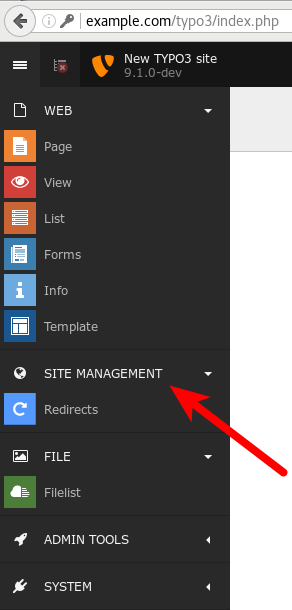
\includegraphics[width=0.45\linewidth]{BackendUserInterface/AddedNewMainModuleSiteManagement.png}
			\end{figure}
		\end{column}
		\begin{column}{.5\textwidth}
			La nuova estensione di sistema \texttt{EXT:redirects} costituisce il primo componente 
			di questo modulo (vedi pagina seguente per dettagli).
		\end{column}
		\begin{column}{.1\textwidth}
		\end{column}
	\end{columns}

\end{frame}

% ------------------------------------------------------------------------------
% LTXE-SLIDE-START
% LTXE-SLIDE-UID:		1bc07d7d-0ca0b392-db7e974f-2d466b5c
% LTXE-SLIDE-ORIGIN:	8bd6b85d-ed8c77e3-94a40b39-e15bb504 English
% LTXE-SLIDE-TITLE:		System Extension "Redirects" Has Been Added
% LTXE-SLIDE-REFERENCE:	Feature-83631-SystemExtensionRedirectsHasBeenAdded.rst
% ------------------------------------------------------------------------------

\begin{frame}[fragile]
	\frametitle{Interfaccia utente Backend}
	\framesubtitle{Redirects}

	Il nuovo modulo permette agli integratori ed editori di configurare i redirect.
	La funzionalità comprende anche un semplice contatore di visite (deve essere abilitato)
	e i rendirizzamenti possono essere impostati come illimitati o per un periodo specifico di tempo

	\begin{figure}
		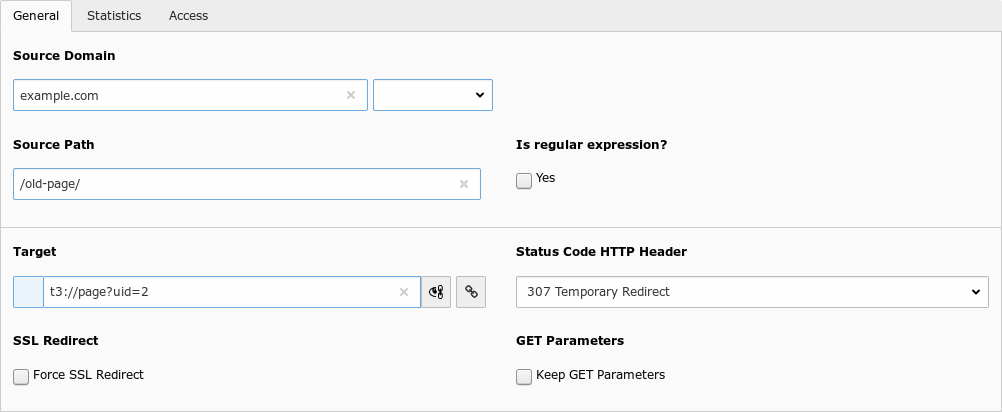
\includegraphics[width=0.8\linewidth]{BackendUserInterface/SystemExtensionRedirectsHasBeenAdded.png}
	\end{figure}

\end{frame}

% ------------------------------------------------------------------------------
% LTXE-SLIDE-START
% LTXE-SLIDE-UID:		f9f13f4b-b7dce235-aee959a0-99301582
% LTXE-SLIDE-ORIGIN:	e10a0f89-e91ecdb3-928841b6-1a84fc50 English
% LTXE-SLIDE-TITLE:		Show Fieldname Next To Title In Debug Mode
% LTXE-SLIDE-REFERENCE:	Feature-83461-ShowFieldnameNextToTitleInDebugMode.rst
% ------------------------------------------------------------------------------

\begin{frame}[fragile]
	\frametitle{Interfaccia utente Backend}
	\framesubtitle{Nomi dei campi in modalità debug}

	\begin{itemize}

		\item Gli integratori e sviluppatori di TYPO3 spesso interagiscono con i campi di backend, ad es.
		quando si impostano i permessi di accesso durante la configurazione di TSConfig.

		\item Invece di esaminare il codice sorgente del browser, i nomi dei campi vengono mostrati
		per ogni campo generato da FormEngine.

		\item Questo vale solo per gli utenti con privilegi di amministratore e richiede che la modalità
			di debug sia abilitata in TYPO3:

			\smaller
				\texttt{\$GLOBALS['TYPO3\_CONF\_VARS']['BE']['debug']}
			\normalsize

	\end{itemize}

	\begin{figure}
		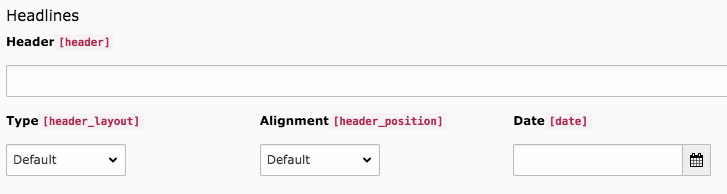
\includegraphics[width=0.60\linewidth]{BackendUserInterface/ShowFieldnameNextToTitleInDebugMode.png}
	\end{figure}

\end{frame}

% ------------------------------------------------------------------------------
